\documentclass[10pt]{article}
\usepackage{icmlko}

\icmlmeta{IP 파운데이션 월드모델}{63}{등급이 자의적이지 않았다}{오래 열려 있던 라벨 위생 항목을 닫는다 --- 개별 결함은 성능에 안 보이고, 신뢰 등급만 방향이 맞다}

\begin{document}

\twocolumn[
\icmlheader

\begin{abstract}
노트 1--8에서 팝업 라벨의 계수 기준과 스코프를 검증하며 레코드마다 신뢰 등급을
매겼다. 그때 남긴 미해결 항목이 예순 노트 동안 열려 있었다. 여섯 도메인 상태에서
닫는다. 먼저 확인한 것 --- \textbf{내부 팝업 레코드는 위생 정보가 이미 충분히
붙어 있다.} 레코드마다 신뢰 등급과 근거, 측정 도구, 라벨 기간과 일별 합 일치
여부, 원본 문서 인용이 있다. 분석 풀 75건의 등급은 \textbf{A가 53건, B가
15건이고 C 이하가 없다}. 미해결 세 건 중 둘은 이미 풀에서 걸러졌고 하나만
남아 있었다(일별 합 불일치). 그다음 검정 --- 결함이 있는 레코드를 빼면 성능이
오르는가. \textbf{개별 결함은 안 보인다} --- 일별 합 불일치 한 건을 빼면
$-$0.0002, 기간 불연속 일곱 건을 빼면 $-$0.0001이다. 그런데 \textbf{신뢰 등급
B 열다섯 건을 빼면 $+$0.0096 오른다} --- 표본을 20\% 버리는데도. 짝지은 구간이
{[}$-$0.012, $+$0.028{]}로 0을 포함해(P$=$0.820) \textbf{채택하지 않았지만},
방향이 맞다는 것 자체가 결과다. \textbf{예순 노트 전에 사람이 매긴 등급이
지금 예측력과 같은 방향을 가리킨다.} 등급 체계가 자의적이지 않았다는 뜻이다.
\end{abstract}
]

\section{오래 열려 있던 항목}

노트 1--8은 팝업 라벨을 다뤘다 --- 계수 기준이 입장인지 참여인지 주최 측
발표인지, 수치의 스코프가 단일 행사인지 합산인지, 출처가 무엇인지. 그 과정에서
레코드마다 신뢰 등급을 매겼고 미해결 항목을 남겼다.

여섯 도메인이 되고 판정 도구가 여러 번 바뀐 지금 다시 본다.

\begin{table}[t]
\centering\tsize
\caption{내부 팝업 레코드에 붙어 있는 위생 정보.}
\begin{tabular}{ll}
\toprule
필드 & 내용 \\
\midrule
\texttt{label\_trust} & 등급과 근거 문장 \\
\texttt{measurement\_instrument} & 현장 웨이팅 로그 등 \\
\texttt{label\_scope} & 기간 · 일수 · 연속성 · 일별 합 일치 \\
\texttt{provenance} & 원본 문서 · 인용 · 열람 기록 \\
\texttt{label\_history} & 변경 이력 \\
\bottomrule
\end{tabular}
\end{table}

\begin{table}[t]
\centering\tsize
\caption{분석 풀 75건의 신뢰 등급.}
\begin{tabular}{lr}
\toprule
A & 53건 \\
B & 15건 \\
C 이하 & 0건 \\
\midrule
원본 미매칭 & 7건 \\
\bottomrule
\end{tabular}
\end{table}

미해결 세 건 중 둘(출처 없음, 디지털 대리 지표)은 계수 기준 필터에서 이미
걸러져 분석 풀에 없다. 하나만 남아 있었다 --- 일별 합이 총계와 안 맞는 건이다.

\section{개별 결함은 성능에 안 보인다}

\begin{figure}[t]
\centering
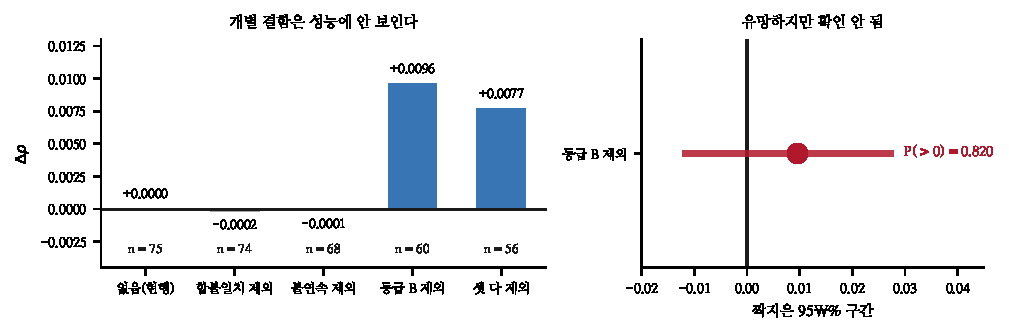
\includegraphics[width=\textwidth]{figs/hygiene.pdf}
\caption{왼쪽 --- 위생 필터별 성능. 오른쪽 --- 등급 B 제외의 구간.}
\end{figure}

\begin{table}[t]
\centering\tsize
\caption{결함 레코드를 뺐을 때.}
\begin{tabular}{lrrr}
\toprule
필터 & 팝업 n & $\rho$ & $\Delta$ \\
\midrule
없음(현행) & 75 & $+$0.3506 & --- \\
일별 합 불일치 제외 & 74 & $+$0.3504 & $-$0.0002 \\
기간 불연속 제외 & 68 & $+$0.3504 & $-$0.0001 \\
\textbf{등급 B 제외} & 60 & $+$0.3602 & \textbf{$+$0.0096} \\
셋 다 제외 & 56 & $+$0.3583 & $+$0.0077 \\
\bottomrule
\end{tabular}
\end{table}

일별 합 불일치와 기간 불연속은 성능에 흔적이 없다. 각각 한 건과 일곱 건인데
빼도 소수점 넷째 자리에서만 움직인다.

\textbf{등급 B를 빼면 $+$0.0096 오른다.} 표본을 75에서 60으로 20\% 줄이는데도
오른다는 것이 요점이다 --- 표본이 줄면 보통 나빠진다.

\section{그런데 채택하지 않는다}

\begin{table}[t]
\centering\tsize
\caption{등급 B 제외의 짝지은 붓스트랩.}
\begin{tabular}{lr}
\toprule
$\Delta\rho$ & $+$0.0096 \\
95\% 구간 & $[-0.012,\ +0.028]$ \\
P($>$0) & 0.820 \\
\midrule
판정 & \textbf{보류} \\
\bottomrule
\end{tabular}
\end{table}

노트 44 이후의 기준대로 구간이 0을 포함하면 채택하지 않는다. 그리고 여기서는
표본 20\%를 버리는 대가가 확실한데 이득이 불확실하다.

\claimx{개별 위생 결함(일별 합 불일치 · 기간 불연속)은 전이 성능에 보이지 않는다.
신뢰 등급만 방향이 맞다 --- B를 빼면 $+$0.0096 오르지만 구간이 0을 포함한다.}
{팝업이 75건이라 어떤 부분집합 실험도 검정력이 낮다. 표본이 두 배가 되면 이
$+$0.0096이 갈릴 것이다.}

\section{등급이 자의적이지 않았다}

이것이 이 노트의 진짜 결과다.

\begin{quote}\fontsize{9.5}{11.5}\selectfont
등급은 예순 노트 전에, 전이 실험이 있기 훨씬 전에, 사람이 출처와 계측 방식을
읽고 매긴 것이다. 그 등급이 지금 \emph{전이 예측력}과 같은 방향을 가리킨다.
확인은 안 됐지만 부호가 맞고, 개별 결함 지표들은 부호조차 안 맞는다.
\end{quote}

라벨 품질을 사람이 판단한 것이 기계적 결함 지표보다 낫다는 뜻이며, 노트 49에서
팝업 축 태깅이 위키백과를 이긴 것과 같은 방향이다. \textbf{이 프로젝트에서
사람이 읽어 매긴 값은 두 번 다 자동 지표를 이겼다.}

\section{한계}

\begin{itemize}[leftmargin=1.1em,itemsep=0.15em]
\item 75건 중 7건은 원본 레코드를 못 찾아 등급을 모른다. 그 7건이 어느 쪽인지에
      따라 결과가 흔들린다.
\item 등급 A와 B의 구분 기준을 이 노트에서 다시 검토하지 않았다. 노트 1--8의
      정의를 그대로 썼다.
\item 측정 도구가 안 적힌 레코드가 60건이 넘는다. 등급은 A인데 도구가 없는
      경우가 많아, 그 필드는 위생 지표로 쓸 수 없다.
\item 다른 다섯 도메인의 라벨 위생은 보지 않았다. 전부 기계 수집이라 사람
      등급이 없다.
\item 미해결 세 건을 ``닫는다''고 했지만 실제로는 둘이 이미 필터에 걸려 있었고
      하나는 성능에 안 보인다는 것을 확인한 것이다. 원인을 고친 것이 아니다.
\end{itemize}

\section{다음}

\begin{enumerate}[leftmargin=1.3em,itemsep=0.15em]
\item 원본을 못 찾은 7건의 등급을 확인한다.
\item 웹툰 전체 수집 완료 후 전면 재측정(2,006/3,973 진행 중).
\item 팝업 표본이 두 배가 되면 등급 B 제외를 다시 판정한다.
\item 측정 도구 필드를 채우거나 버린다. 지금은 있으나 마나다.
\end{enumerate}

\vspace{0.6em}
\hrule height 0.3pt
\vspace{0.5em}
{\footnotesize
\textbf{참고문헌}\\[0.3em]
Kaufman, S., Rosset, S., Perlich, C. (2012). Leakage in data mining.
\emph{ACM TKDD}, 6(4), 1--21.\\[0.15em]
Efron, B., Tibshirani, R. J. (1993). \emph{An Introduction to the Bootstrap}.
Chapman \& Hall.\\[0.15em]
Krippendorff, K. (2004). \emph{Content Analysis: An Introduction to Its
Methodology}, 2nd ed. Sage.\\[0.15em]
Northcutt, C. G., Athalye, A., Mueller, J. (2021). Pervasive label errors in test
sets. \emph{NeurIPS D\&B}.\\[0.15em]
Ben-David, S. et al. (2010). A theory of learning from different domains.
\emph{Machine Learning}, 79(1--2), 151--175.
}

\end{document}
